\documentclass[conference,double column]{IEEEtran}
\usepackage[a4paper,left=2.54 cm,right=2.54 cm,top=2.54 cm,bottom=2.54 cm]{geometry}
\usepackage{graphicx}
\usepackage{cite}
\usepackage{epstopdf}
\usepackage{amsmath,amssymb,amsfonts}
\usepackage{algorithmic}
\usepackage{graphicx}
\usepackage{textcomp}
\usepackage{xcolor}
\def\BibTeX{{\rm B\kern-.05em{\sc i\kern-.025em b}\kern-.08em
		T\kern-.1667em\lower.7ex\hbox{E}\kern-.125emX}}
\epstopdfDeclareGraphicsRule{.pdf}{.png}
\DeclareGraphicsExtensions{.png,.pdf}


\begin{document}
	\title{Is Cyber Security Smart Enough Against Cyber Crime?}
	\author{\IEEEauthorblockN{	Md Shabir Khan Akash  \\Roll: 1603108 \\Computer Science \& Engineering\\RUET\\ \and  Md Shohanoor Rahman\\Roll: 1603112\\Computer Science \& Engineering\\RUET}}
	
	\maketitle
	
	
	\begin{abstract}
		The topic that we are interested to discuss and focus on our technical writing is involved with the term “Cyber Security”. This term is quite familiar in the era of this digital world and modern technology. Cyber Security is the protection or shield against the term ‘Cybercrime’ that is defined as a crime in which a computer is the object of the crime (unethical hacking, phishing, spamming) or is used as a tool to commit an offense (cyber bullying, hate crimes). Cyber Security can possess the potential of removing cyber crime from the cyber world, but sometimes cyber security also lags behind from taking necessary steps against cyber crime. Unfortunately, there's no 100\% guarantee that even with the best precautions some of these cyber crimes won't happen to you, but there are steps that can be taken to minimize the chances.
	\end{abstract}
	
	\begin{IEEEkeywords}
		cybercrime, phishing, cybersecurity, DDoS attack, ransomware, unethical hacking, Anti-malware software, survey, security, encryption
	\end{IEEEkeywords}
	
	\section{Introduction}		
	In the most basic sense, cybersecurity refers to the protection of computer systems from the theft of or damage to their hardware, software, or electronic data, as well as from the disruption or misdirection of the services they provide.~\cite{r1}.The field is becoming more important due to increased reliance on computer systems, the Internet~\cite{r2} and wireless network standards such as Bluetooth and Wi-Fi, and due to the growth of "smart" devices, including smartphones, televisions, and the various devices that constitute the "Internet of things". Owing to its complexity, both in terms of politics and technology, cybersecurity is also one of the major challenges in the contemporary world.~\cite{r3} Cybersecurity includes both physical preventive measures as well as digital.So as example,
	\begin{itemize}
		\item Physical forms of cybersecurity: Locked doors and video surveillance systems, Security Sensor Vaults etc.
		\item Digital forms of cybersecurity: Antivirus softwares, Network monitoring services, data encryption, Cryptography etc.
	\end{itemize}		
	
	Cyber security is the name for the safeguards taken to avoid or reduce any disruption from an attack on data, computers or mobile devices. Cyber security covers not only safeguarding confidentiality and privacy, but also the availability and integrity of data, both of which are vital for the quality and safety of care. Security breaches can occur when we use paper records, send information using fax machines and even verbally. However, the consequences of security breaches with digital information are potentially far more severe, as information can be distributed more easily and to a far wider audience.
	
	
	Cybercrime generally occurs with that internet user who doesn't really concern or care about cyber security. As from the cybercrime perspective, Hackers are one of the real culprits of this notorious activities. From the cyberbullying to unethical hacking, Online Money theft each and every cybercrimes of the day to day modern life are quite interrelated.Cybercrimes are classified into some types by their activity and consequences.Computer or cybercrime encompasses a broad range of activities~\cite{r4}. These are- 
	\begin{itemize}
		\item Financial fraud crimes
		\item Cyberterrorism
		\item Cyberextortion
		\item Cyberwarfare
		\item Online harassment
		\item Drug trafficking
		\item Spreading Offensive content
	\end{itemize}
	
	Though there are enormous number of cybercrimes up there on the web but proper learning about web, some precautions made by the internet user can certainly make the bad things disappeared right away.  
	
	\section{Literature review}
	Several definitions of the terms cyber-attack, cyber-crime, etc. can be found among the international literature, all
	having in common the aim to compromise the confidentiality, integrity and availability of data. The technological
	evolution also brings along the progress of cyber-crime, thus new ways to perform attacks, reach to even harder to
	penetrate targets and remain untracked are developed continuously. However, traditional cyber threats remain as the
	source of the most common attacks. Various types of attacks have been defined and studied among the international
	literature:
	
	\begin{itemize}
		\item Man in the middle attack occurs when the attacker interferes between the two communication ends, thus
		every message sent from source A to source B reaches the attacker before reaching its destination. The
		risks further posed by this type of attack comprise of unauthorised access to sensitive information or
		possibilities to alter the information/message that reaches the destination by the attacker
		\item A DoS or DDoS attack is analogous to a group of people crowding the entry door of a shop, making it hard for legitimate customers to enter, thus disrupting trade.
		
		Criminal perpetrators of DoS attacks often target sites or services hosted on high-profile web servers such as banks or credit card payment gateways. Revenge, blackmail~\cite{r5} and activism~\cite{r6} can motivate these attacks,
		\item Brute force attack comprises of repeated attempts to gain access to protected information (e.g. passwords,
		encryption, etc.) until the correct key is found, and information can thus be reached
		\item Social engineering is the general term that describes techniques used to gain unauthorized access to
		information through human interaction.
		\item Phishing is a technique aiming to steal private information from users through masquerading as a trustful
		source like using a clone website of a trusted site or using any subdomain of any famous reliable company etc.
	\end{itemize}
	
	\section{Methodology}
	Cyber security is a constantly changing area and moreover often it may seem quite confusing. However, there are quite many effective and relatively simple steps that can be taken to protect information and protect a user and his/her organization.By Taking some simple and effective actions and practicing safe behaviors will reduce online threats as well as cybercrimes.\\
	
	
	Some effectively important steps to improve cyber security are the following:
	\subsection{MOVING AWAY FROM USING UNSUPPORTED SOFTWARE}
	This is when software e.g. operating systems,apps,web browsers etc. are no longer updated by the supplier. Although the software will continue to operate, it will no longer protect against online threats through updates or patching (a software update, often relates to improving security). If a security weakness is discovered, software can be compromised and become vulnerable to a cyber-attack. For benefits to be gained from up-to-date security measures, such as improved speed and efficiency, only use supported software on your systems and devices. If unsupported software is being used, ensure that properly manage the risk by having a strong firewall and up-to-date anti-virus and/or anti-malware software.
	\subsection{MANAGING SECURITY RELATIONSHIPS WITH SUPPLIERS AND PARTNERS}
	As organisation grows and works with more suppliers and partners,there become a link in one or more complex supply chains.It is important to observe good practice (and in many cases, compliance) because vulnerabilities will place not only own organisation at risk, but also others within the supply chain. If use third-party managed IT services, contracts and service level agreements should be checked, and ensure that whoever handles systems and data has security controls in place.
	\subsection{BACKING UP OWN DATA}
	Safeguard of most important data by  backing up to a secure external hard drive or storage system based  in the Cloud. There also ensure regularly test back-ups and, if confidential data off-site e.g. the Cloud be saved,all appropriate data protection measures and government standards and guidance that relate to health and social care organisations must be followed.
	\subsection{USING STRONG PASSWORDS}
	Passwords should be easy to remember and difficult to guess.Numbers and symbols can still be used but using three random words is the key to creating a strong password.Using a strong, separate password for email and other important accounts is a good practice.For most important accounts, if it’s available, there should use Two-Factor Authentication. This means involving a second step after entering your password e.g. providing a fingerprint, answering a security question, or entering a unique code sent to users device. 
	\subsection{RUNNING UP-TO-DATE ANTI-VIRUS SOFTWARE}
	Computers, tablets and smartphones can easily become infected by small pieces of software known as malware. Common types include viruses or spyware and ransomware. To help prevent infection, install internet security software, like anti-virus and/or anti-malware on devices and keep it up to date. 
	\subsection{TRAINING STAFFS OR FRIENDS TO BE CYBER AWARE}
	Make sure staff are trained to know the benefits of operating digitally, but are also aware of cyber security threats and how to deal with them. Due to the rapid development and changes in digital technology it is a good idea to add cyber security to annual training plans/ matrix. 
	\subsection{DELETEING SUSPICIOUS EMAILS AND AVOID CLICKING ON UNKNOWN ATTACHMENTS OR LINKS}
	Email is an excellent communication tool but is frequently used to deliver unwanted or unwelcome material, often referred to as ‘spam’ or ‘junk’ email. Avoiding respond to such ‘phishing’ emails even if they seem to come from a company or person may be known, because doing so can confirm the address is legitimate to the sender. 
	\subsection{ALWAYS DOWNLOADING AND INSTALLING THE LATEST SOFTWARE AND APP UPDATES}
	Software updates are designed to fix weaknesses in software and apps which could be used by hackers to attack on device. Installing them as soon as possible helps to keep the device secure.
	
	\section{Statistical Data}
	\subsection{Statistical Data on Various Cyber Crimes}
	Phishing is the fraudulent attempt to obtain sensitive information such as usernames, passwords and credit card details by disguising oneself as a trustworthy entity in an electronic communication.~\cite{r7} Typically carried out by email spoofing or instant messaging, it often directs users to enter personal information at a fake website which matches the look and feel of the legitimate site.~\cite{r8}
	
	
	“Domain names” are defined as second-level domain names, plus third-level domain names if the
	relevant registry offers third-level registrations.~\cite{r9} An example is the .CN (China) registry, which offers
	both second-level registrations and third-level registrations(in zones such as com.cn, gov.cn, zj.cn,
	etc.)
	
	
	Basic statistical data table on Phishing Attacks and Domains Used ranging a time period of 2012-2016 is given below- 
	
	
	\begin{table}[!h]
		\renewcommand{\arraystretch}{1.3}
		\caption{Basic statistical data table on Phishing Attacks and Domains(2013-2016)~\cite{r10}}
		\label{table1}
		\centering
		\begin{tabular}{|c|c|c|c|c|}
			\hline
			% after \\: \hline or \cline{col1-col2} \cline{col3-col4} ...
			& 2013 & 2014 & 2015 & 2016 \\
			\hline
			Phishing Domain& 135,848 & 183,222 & 160,155 & 195,475 \\
			\hline
			Attacks & 188,323 & 247,713 & 227,471 & 255,065 \\
			\hline
			TLDs & 223 & 288 & 355 & 454 \\
			\hline
			new gTLDs & 0 & 72 & 120 & 228 \\
			\hline
			IP-based phish & 4,366 & 6,472 & 2,245 & 5,378 \\
			\hline
			Harmful Domains
			& 35,004 & 49,932 & 34,102 & 95,424 \\
			\hline
		\end{tabular}
	\end{table}
	
	\begin{center}
		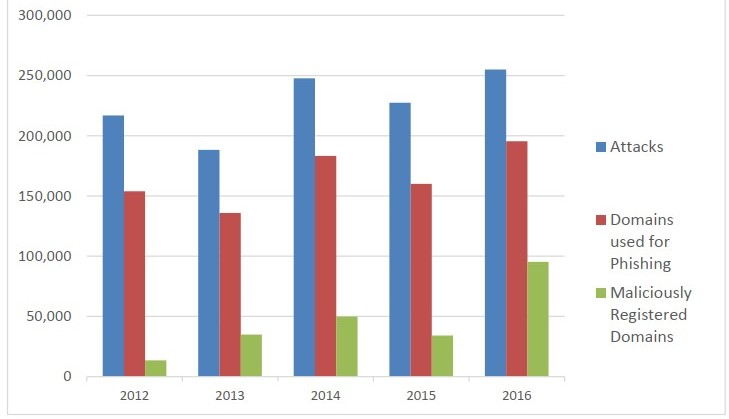
\includegraphics[scale=0.40]{phishAttack.jpg}
		{\footnotesize Figure 1: Phishing Attacks and Domains Used (2012-2016)~\cite{r10}}
	\end{center}
	
	
	Phishing attacks on cyber-world can be performed in various ways by some cyber criminals also known as Hackers.In June 2012, attackers compromised Distributed Denial of Service(DDoS) mitigation service on CloudFlare by using flaws in AT\&T's voicemail service for its mobile users; similarly, Google's account-recovery service for its Gmail users~\cite{r11}. Almost in every year, a handsome amount of attacks keep increasing in the cyber world. Some are done by hackers and some with domain cloning. Domain cloning is like the cloning a trustworthy, popular domain but the cloned domain is malicious domain used for mischief on web by hackers. A recent statistical research~\cite{r10} published a graphical representation of phishing attacks by resources based on the period from 2009 to 2016.
	
	
	\begin{center}
		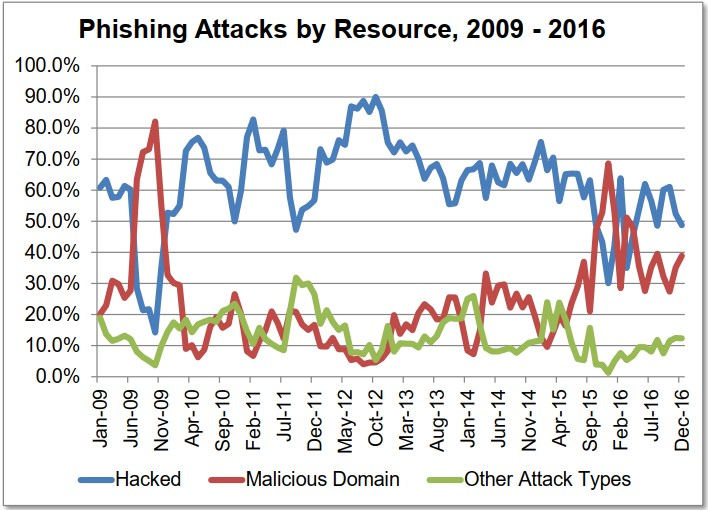
\includegraphics[scale=0.40]{maldom.jpg}
		{\footnotesize Figure 2: Phishing Attacks by resource (2009-2016)~\cite{r10}}
	\end{center}
	
	
	Along with Phishing attacks there are many other types of tools are used to perform cyber crimes. These are generally known as Trojans, Virus, Worms, Rogueware, Ransomware, Adware and many others. A little Carelessness can result in very horrible situation which is not a good thing at all. A relative proportions of the types of new malware samples identified in the later half of 2012 reported by Anti-Phishing group in Figure 3~\cite{r12}. That pie chart report is presented below-
	
	
	\begin{center}
		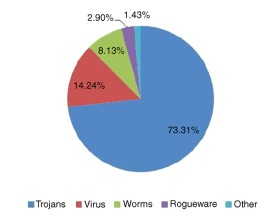
\includegraphics[scale=0.90]{ccother.jpg}\\
		{\footnotesize Figure 3: Types of Malware~\cite{r11}}
	\end{center}
	
	\subsection{Statistical Data on Cyber Security}
	As per there is a wide range of cyber crimes and tools are present to make these notorious crimes in live action, the term "Cyber security" is also there for protection against this.Antivirus is one the most commonly used programs which is used for protecting the system from malicious cyber attacks.A famous antivirus company named "Kaspersky" made a geographical survey on crypto-ransomware attacks on their official bulletin~\cite{r13}.	
	
	
	\begin{center}
		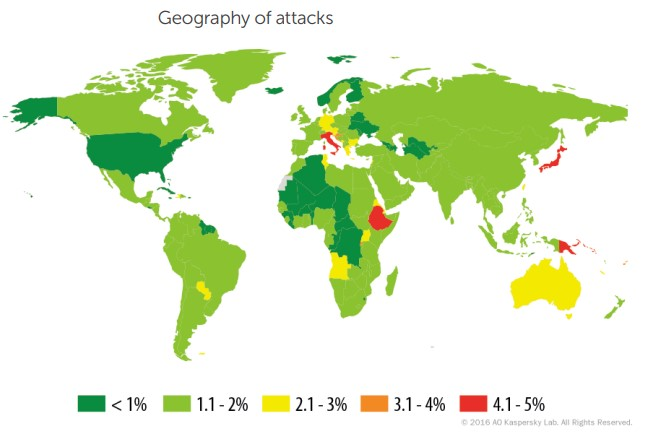
\includegraphics[scale=0.46]{geocra.jpg}\\
		{\footnotesize Figure 4: Geography of crypto-ransomware attacks in 2016 (percentage of targeted users)~\cite{r13}}
	\end{center}
	
	That geographical survey of Figure 4 makes a clear impression on the percentage of crypto-ransomware attack.From the Figure IV,around 4.1\%-5\% in Northern European,Middle-Eastern African region, Western Australia, Eastern Asia and around 2.1\%-3\% in Australia,Europe,Southern Africa and middle portion of South America.  
	
	
	Recently OPSWAT an organization discussing and working to eliminate malware and zero-day attacks with their efforts. They provided a survey on various antivirus by their market share till January 2019. 
	
	
	\begin{center}
		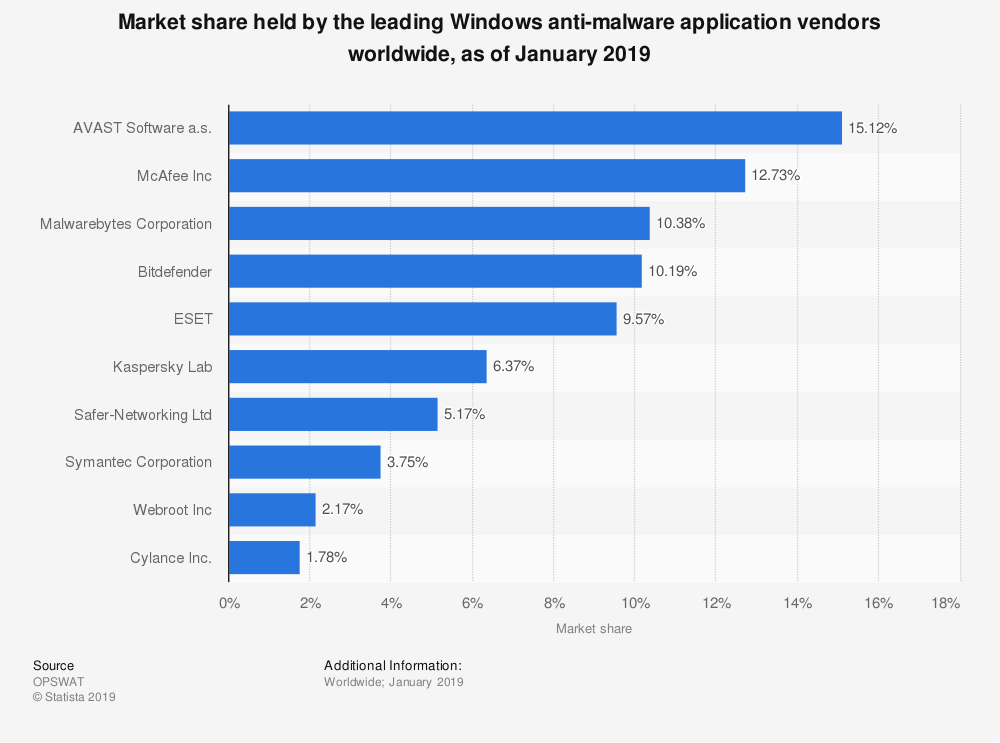
\includegraphics[scale=0.22]{antivsurvey.png}\\
		{\footnotesize Figure 5: Survey on Antivirus Users till January 2019~\cite{r14}}
	\end{center}
	
	The bar chart in Figure 5 generally is indicating the percentage of market share of different wel-known windows anti-malware applications. If the survey is analyzed carefully then, it can be observed that, Avast Software, McAfee Inc, Malwarebytes Corporation, Bitdefender, ESET are the top 5 anti-malware companies that held the market share till january 2019. Moreover their market share was ranging from 10\% to 15\% which is quite good. This makes a general idea about the trust of internet users on these anti-malware software companies.\\
	
	\section{Result Analysis}
	So based on the analysis of the above statistical data on both cybercrime and cybersecurity, it can be said in the end that, cyber crimes are emerging at a high rate of growth which is a very threatening situation. Though nowadays cybersecurity systems are advancing way to quickly to the betterment of cyberspace and with the aim of ensuring a safe and secure internet experience to all the users, but it is a matter of regret that still some third world countries' people aren't aware of these cybercrimes even it is as much sensitive as any other crimes around us. A proper cautious mind and ability to make the right and efficient decision can fetch the secure internet experience.
	
	
	\section{Future Works} 
	Though cybersecurity is upgrading itself quite in a good pace, there needs to be done some future research or upgrading works which can ensure much safety and secure environment. Some important points that can be kept in a side for future work on this topic. These are -
	
	
	\subsection{Ensuring a safer internet for upcoming generation}
	The upcoming generations are the future of our society and country. If our next generation gets hit by the wrong side of internet, becomes virtually addicted and not participating in productive and educative competition then that nation or country will be at stake. So for the betterment, ensuring safer internet for new generation is a must.
	
	\subsection{Increasing the development of trustworthy software}
	It's quite natural that a person or internet user will continue to use his/her that very product/software/application which he/she finds trustworthy. So gaining trust is quite huge tough task. Every software development company needs to do this tough work for its own good as well as safer internet. So trustworthy companies need to be widespread its branches.
	
	\subsection{Developing Security System}
	One of the most important future research work can be done on this topic is to find or research about more and more efficient way of securing data. Data is one of most valuable items in this 21st century. So securing the data is a very challenging task which needs to be keeping in mind for the future research or work purposes.
	
	
	\section{Conclusion} 
	
	
	\bibliography{refers} 
	\bibliographystyle{ieeetr}
	
\end{document}